\documentclass{beamer}

\usepackage{amsmath, amssymb}
\usepackage{tikz-cd}
\usepackage{xcolor}
\usepackage{graphicx}

\title{MAT414 - Modern Algebra}
\subtitle{Isomorphisms \cite{JAG2017}}
\author{\textbf{Miraj Samarakkody}}
\institute{Tougaloo College}
\date{Updated - \today}

\begin{document}

\begin{frame}
    \titlepage
\end{frame}




\begin{frame}
    \frametitle{Motivation}

    Counting objects..... 

\end{frame}

\begin{frame}
    \frametitle{Group Isomorphism}

    \begin{block}{Definition}
        An \textit{Isomorphism} \(\phi\) from a group \(G\) to a group \(\overline{G}\) is a bijective mapping such that:
        \[
            \phi(ab) = \phi(a)\phi(b) \quad \forall a,b \in G
        \]
        If there is an isomorphism from \(G\) to \(\overline{G}\), we say that \(G\) and \(\overline{G}\) are \textit{isomorphic} and write \(G \cong \overline{G}\).
    \end{block}

\end{frame}

\begin{frame}
    \frametitle{Example}

    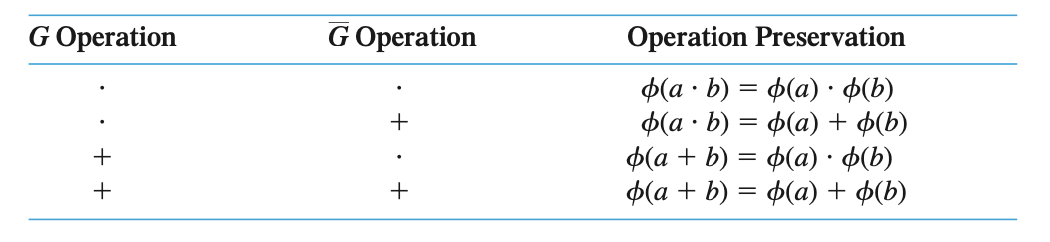
\includegraphics[scale=0.6]{Figures/fig_6.png}

\end{frame}

\begin{frame}
    \frametitle{Steps to Prove Isomorphism}

    \begin{enumerate}
        \item ``Mapping.'' Define a candidate for the isomorphism; that is, define a function \(\phi: G \to \overline{G}\).\pause
        \item ``Injective.'' Show that \(\phi\) is injective (one-to-one). That is, assume that \(\phi(a)=\phi(b)\) and prove that \(a=b\).\pause 
        \item ``Surjective.'' Show that \(\phi\) is surjective (onto). That is, show that for every \(b \in \overline{G}\), there exists an \(a \in G\) such that \(\phi(a)=b\).\pause
        \item ``O.P.'' Prove \(\phi\) is operation-preserving. That is, show that \(\phi(ab)=\phi(a)\phi(b)\) for all \(a,b \in G\).
    \end{enumerate}

\end{frame}


\begin{frame}
    \frametitle{Example 1}

    Let \(G\) be the real numbers under addition, and let \(\overline{G}\) be the positive real numbers under multiplication. Prove that the \(G\) and the \(\overline{G}\) isomorphic under the mapping \(\phi(x)=2^x\). 

\end{frame}

\begin{frame}
    \frametitle{Example 2}

    Any infinte cyclic group is isomorphic to \(\mathbb{Z}\). 

\end{frame}

\begin{frame}
    \frametitle{Example 3}

    Prove that the mapping from \(\mathbb{R}\) under addition to itself given by \(\phi(x)=x^3\) is not an isomorphism.

\end{frame}

\begin{frame}
    \frametitle{Example 4}

    Prove that \(U(10) \cong \mathbb{Z}_4\) and \(U(5)\cong \mathbb{Z}_4\). 

\end{frame}

\begin{frame}
    \frametitle{Example 5}

    Prove that there is no isomorphism from \(\mathbb{Q}\), the group of rational numbers under addition, to \(\mathbb{Q}^*\), the group of non-zero rational numbers under multiplication. 

\end{frame}

\begin{frame}
    \frametitle{Example 6}

    Let \(G=SL(2, \mathbb{R})\), the group of \(2 \times 2\) real matrices with deteminant 1. Let \(M\) be any \(2 \times 2\) real matrix with determinant 1.  

\end{frame}


\begin{frame}
    \frametitle{References}
    \bibliographystyle{plain} % or another style like unsrt, alpha, etc.
    \bibliography{reference}  % omit the .bib extension
\end{frame}

\end{document}